\documentclass[tikz,border=2pt]{standalone}
\usepackage{amsmath,amssymb}
\usepackage{tikz}

\begin{document}
% First fit on the items 15, 30, 20, 35 (capacity 50) in the given order: 15 -> container 1,
% 30 -> container 1 (45), 20 does not fit (65) -> container 2, 35 fits neither -> container 3.
% Three containers, although two suffice.
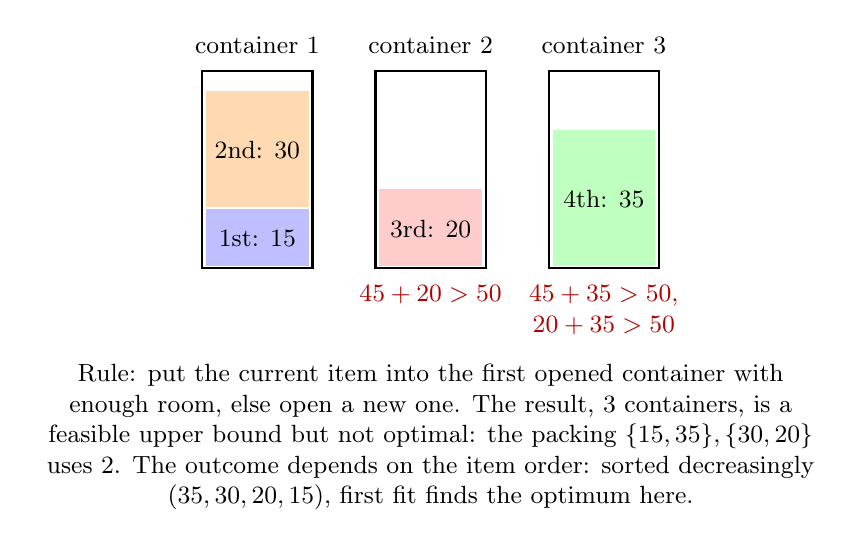
\begin{tikzpicture}[every node/.style={font=\small}, y=0.05cm]
	\foreach \x/\n in {0/1, 2.2/2, 4.4/3} {
		\draw[thick] (\x,0) rectangle ({\x+1.4},50);
		\node[anchor=south] at ({\x+0.7},52) {container \n};
	}
	\fill[blue!25] (0.05,0.5) rectangle (1.35,15); \node at (0.7,7.5) {1st: $15$};
	\fill[orange!30] (0.05,15.5) rectangle (1.35,45); \node at (0.7,30) {2nd: $30$};
	\fill[red!20] (2.25,0.5) rectangle (3.55,20); \node at (2.9,10) {3rd: $20$};
	\fill[green!25] (4.45,0.5) rectangle (5.75,35); \node at (5.1,17.5) {4th: $35$};
	\node[red!70!black, anchor=north] at (2.9,-2) {$45+20>50$};
	\node[red!70!black, anchor=north, align=center] at (5.1,-2) {$45+35>50$,\\ $20+35>50$};
	\node[anchor=north, align=flush center, text width=10cm] at (2.9,-22) {Rule: put the current item into the first opened container with enough room, else open a new one. The result, $3$ containers, is a feasible upper bound but not optimal: the packing $\{15,35\},\{30,20\}$ uses $2$. The outcome depends on the item order: sorted decreasingly ($35,30,20,15$), first fit finds the optimum here.};
\end{tikzpicture}
\end{document}
